
%%%%%%%%%%%%%%%%%%%%%%%%%%%%%%%%%%%%%%%%%%%%%%%
%%%     Declarations (skip to Begin Document, line 112, for parts you fill in)
%%%%%%%%%%%%%%%%%%%%%%%%%%%%%%%%%%%%%%%%%%%%%%%

\documentclass[10pt]{article}

\usepackage{geometry}  % Lots of layout options.  See http://en.wikibooks.org/wiki/LaTeX/Page_Layout
\geometry{letterpaper}  % ... or a4paper or a5paper or ... 
\usepackage{fullpage}  % somewhat standardized smaller margins (around an inch)
\usepackage{setspace}  % control line spacing in latex documents
\usepackage[parfill]{parskip}  % Activate to begin paragraphs with an empty line rather than an indent

\usepackage{amsmath,amssymb}  % latex math
\usepackage{empheq} % http://www.ctan.org/pkg/empheq
\usepackage{bm,upgreek}  % allows you to write bold greek letters (upper & lower case)

% for typsetting algorithm pseudocode see http://en.wikibooks.org/wiki/LaTeX/Algorithms_and_Pseudocode
\usepackage{algorithmic,algorithm}  

\usepackage{graphicx}  % inclusion of graphics; see: http://en.wikibooks.org/wiki/LaTeX/Importing_Graphics
% allow easy inclusion of .tif, .png graphics
\DeclareGraphicsRule{.tif}{png}{.png}{`convert #1 `dirname #1`/`basename #1 .tif`.png}

\usepackage{xspace}
\newcommand{\latex}{\LaTeX\xspace}

\usepackage{color}  % http://en.wikibooks.org/wiki/LaTeX/Colors

\long\def\ans#1{{\color{blue}{\em #1}}}
\long\def\ansnem#1{{\color{blue}#1}}
\long\def\boldred#1{{\color{red}{\bf #1}}}

% Useful package for syntax highlighting of specific code (such as python) -- see below
\usepackage{listings}  % http://en.wikibooks.org/wiki/LaTeX/Packages/Listings
\usepackage{textcomp}

%%% The following lines set up using the listings package
\renewcommand{\lstlistlistingname}{Code Listings}
\renewcommand{\lstlistingname}{Code Listing}

%%% Specific for python listings
\definecolor{gray}{gray}{0.5}
\definecolor{green}{rgb}{0,0.5,0}

\lstnewenvironment{python}[1][]{
\lstset{
language=python,
basicstyle=\footnotesize,  % could also use this -- a little larger \ttfamily\small\setstretch{1},
stringstyle=\color{red},
showstringspaces=false,
alsoletter={1234567890},
otherkeywords={\ , \}, \{},
keywordstyle=\color{blue},
emph={access,and,break,class,continue,def,del,elif ,else,%
except,exec,finally,for,from,global,if,import,in,i s,%
lambda,not,or,pass,print,raise,return,try,while},
emphstyle=\color{black}\bfseries,
emph={[2]True, False, None, self},
emphstyle=[2]\color{green},
emph={[3]from, import, as},
emphstyle=[3]\color{blue},
upquote=true,
morecomment=[s]{"""}{"""},
commentstyle=\color{gray}\slshape,
emph={[4]1, 2, 3, 4, 5, 6, 7, 8, 9, 0},
emphstyle=[4]\color{blue},
literate=*{:}{{\textcolor{blue}:}}{1}%
{=}{{\textcolor{blue}=}}{1}%
{-}{{\textcolor{blue}-}}{1}%
{+}{{\textcolor{blue}+}}{1}%
{*}{{\textcolor{blue}*}}{1}%
{!}{{\textcolor{blue}!}}{1}%
{(}{{\textcolor{blue}(}}{1}%
{)}{{\textcolor{blue})}}{1}%
{[}{{\textcolor{blue}[}}{1}%
{]}{{\textcolor{blue}]}}{1}%
{<}{{\textcolor{blue}<}}{1}%
{>}{{\textcolor{blue}>}}{1},%
%framexleftmargin=1mm, framextopmargin=1mm, frame=shadowbox, rulesepcolor=\color{blue},#1
framexleftmargin=1mm, framextopmargin=1mm, frame=single,#1
}}{}
%%% End python code listing definitions

%%% Specific for matlab listings
\definecolor{dkgreen}{rgb}{0,0.6,0}
\definecolor{gray}{rgb}{0.5,0.5,0.5}
\definecolor{mauve}{rgb}{0.58,0,0.82}
 
\lstnewenvironment{matlab}[1][]{
\lstset{ %
  language=Matlab,                % the language of the code
  basicstyle=\footnotesize,           % the size of the fonts that are used for the code
  numbers=left,                   % where to put the line-numbers
  numberstyle=\tiny\color{gray},  % the style that is used for the line-numbers
  stepnumber=2,                   % the step between two line-numbers. If it's 1, each line 
                                  % will be numbered
  numbersep=5pt,                  % how far the line-numbers are from the code
  backgroundcolor=\color{white},      % choose the background color. You must add \usepackage{color}
  showspaces=false,               % show spaces adding particular underscores
  showstringspaces=false,         % underline spaces within strings
  showtabs=false,                 % show tabs within strings adding particular underscores
  frame=single,                   % adds a frame around the code
  rulecolor=\color{black},        % if not set, the frame-color may be changed on line-breaks within not-black text (e.g. commens (green here))
  tabsize=2,                      % sets default tabsize to 2 spaces
  captionpos=t,                   % sets the caption-position to top
  breaklines=true,                % sets automatic line breaking
  breakatwhitespace=false,        % sets if automatic breaks should only happen at whitespace
  title=\lstname,                   % show the filename of files included with \lstinputlisting;
                                  % also try caption instead of title
  keywordstyle=\color{blue},          % keyword style
  commentstyle=\color{dkgreen},       % comment style
  stringstyle=\color{mauve},         % string literal style
  escapeinside={\%*}{*)},            % if you want to add LaTeX within your code
  morekeywords={*,...}               % if you want to add more keywords to the set
  framexleftmargin=1mm, framextopmargin=1mm, frame=single,#1 % display caption
} }{}
%%% End matlab code listing definitions

%%%%%%%%%%%%%%%%%%%%%%%%%%%%%%%%%%%%%%%%%%%%%%%
%%%     Begin Document
%%%%%%%%%%%%%%%%%%%%%%%%%%%%%%%%%%%%%%%%%%%%%%%

\begin{document}

\begin{center}
    {\Large {\bf ISTA 421/521 -- Homework 2}} \\
    \boldred{Due: Tuesday, September 30, 10pm} \\
    12 points total Undergraduate / 16 points total Graduate
\end{center}

\begin{flushright}
Emanuel Carlos de Alcantara Valente %% Fill in your name here

Undergraduate %% select which you are!
\end{flushright}

\vspace{1cm}
{\Large {\bf Instructions}}

In this assignment you are required to write 3 scripts in python.  They will be submitted as 3 separate files, although you are free to copy chunks of code from one script to the next as desired.  The names for the script files are specified in problems 1, 5 and 8, below.

Included in the homework 2 release are two sample scripts ({\tt fitpoly\_incomplete.py} and {\tt cv\_demo\_incomplete.py}) and two data files ({\tt womens100.csv}, and {\tt synthdata2014.csv}).  The sample scripts are provided for your convenience -- you may use any part of the code in those scripts for your submissions.  Note that neither will run just as provided: you must fill in the calculation of $\mathbf{w}$.  The data files are provided in {\tt .csv} (comma separated values) format.  The script {\tt fitpoly\_incomplete.py} shows how to load the files.

All problems except problem 1 require that you provide some ``written'' answer (in some cases also figures), so you will also submit a .pdf of your written answers.  (You can use \latex or any other system (including handwritten; plots, of course, must be program-generated) as long as the final version is in PDF.)

\boldred{The final submission will include (minimally) the three scripts and a PDF version of your written part of the assignment.  You are required to create either a .zip or tarball (.tar.gz / .tgz) archive of all of the files for your submission and submit the archive to the d2l dropbox by the date/time deadline above.}

NOTE: Problems 6 and 7 are required for Graduate students only; Undergraduates may complete them for extra credit equal to the point value.

(FCMA refers to the course text: Rogers and Girolami (2012), {\em A First Course in Machine Learning}.  For general notes on using \latex to typeset math, see: {\tt http://en.wikibooks.org/wiki/LaTeX/Mathematics})
\vspace{.5cm}

%%%%%%%%%%%%%%%%
%%%     Problems
%%%%%%%%%%%%%%%%

\newpage
\begin{itemize}

%%%     Problem 1
\item[1.] [2 points]
Adapted from {\bf Exercise 1.2} of FCMA p.35:

Write a Python script that can find the parameters $\mathbf{w}$ for an arbitrary dataset of $x_n, t_n$ pairs.  You will use this script to answer problem 2, which only requires fitting a simple line to the data (i.e., you only need to fit parameters $w_0$ and $w_1$); however, in problems 5 and 8 you will need to fit higher-order polynomial models (e.g., $t = w_0 + w_1x + w_2x^2 + ...$), so it is recommended that your script is generalized to handle higher-order polynomials.  The script {\tt fitpoly\_incomplete.py} is provided to help get you started.  {\tt fitpoly\_incomplete.py} provides helper functions to read data, plot data, and plot the model (once you've determined the weight vector $\mathbf{w}$), but the function for computing linear least-squares fit, fitpoly (starting on line 36), is incomplete -- you need to fill this in -- it takes as input the data vector $\mathbf{x}$, the target values vector $\mathbf{t}$, and the scalar {\tt model\_order}, which is an integer representing the polynomial order of the model; fitpoly is intended to return the $\mathbf{w}$ (column) vector (e.g., as a numpy matrix such as the following:
\begin{verbatim}
>>> m = numpy.matrix([1,2,3]) # this creates a matrix with one row
matrix([[1, 2, 3]]) 
>>> m.transpose()   # transposition makes returns a column vector
matrix([[1],
        [2],
        [3]])
>>> numpy.matrix([[1],[2],[3]]) # or we could specify the column directly
matrix([[1],
        [2],
        [3]])
\end{verbatim}
The above isn't literally the code you'd use, but shows how you can create and transpose matrices, with row and column vectors simply being limiting cases of matrices with one row or 3 rows with 1 value each, respectively).  You will want to look at the numpy package, including the linear algebra package {\tt numpy.linalg}, for linear algebra operators.  Also, you don't have to use {\tt fitpoly\_incomplete.py}; you can write your own script from scratch.  Whichever you choose, your script must have the ability to plot the data with the fitted model.

Just to state the obvious: the objective of this exercise is for you to implement the linear least squares fit solution (i.e., the normal equations) -- in their general matrix form.  {\bf DO NOT} use existing least squares solvers, such as {\tt numpy.linalg.lstsq}, or scikit learn's {\tt sklearn.linear\_model.LogisticRegression}; however, it is certainly fine to use these to help {\em verify} your implementation's output.

You will submit your script as a stand-alone file called {\tt fitpoly.py}.

{\bf Solution:} The code is attached: `fitpoly.py'


\newpage
%%%     Problem 2
\item[2.] [1 point]
Adapted from {\bf Exercise 1.6} of FCMA p.35:

Table 1.3 (p.13) of FCMA lists the women's 100m gold medal Olympic results -- this data is provided in the file {\tt womens100.csv} in the data folder.  Using your script from problem 1, find the 1st-order polynomial model (i.e., a line with parameters $w_0$ and $w_1$) that minimizes the squared loss of this data.  Report the model here as a linear equation and also include a figure that plots your model with the data.

{\bf Solution:}  According to the output of our program from exercise 1:

\begin{verbatim}
[emanuel@localhost submit]$ python fitpoly.py 
Identified model parameters:
[[  4.09241546e+01]
 [ -1.50718122e-02]]
\end{verbatim}

The $w_{0} = 40.924$ and $w_{1} = -0.015$, so the 1st-order polynomial model is going to be: 

\begin{center}$t = 40.924 -0.015x$. \end{center}

\begin{figure}[htb]
\begin{center}
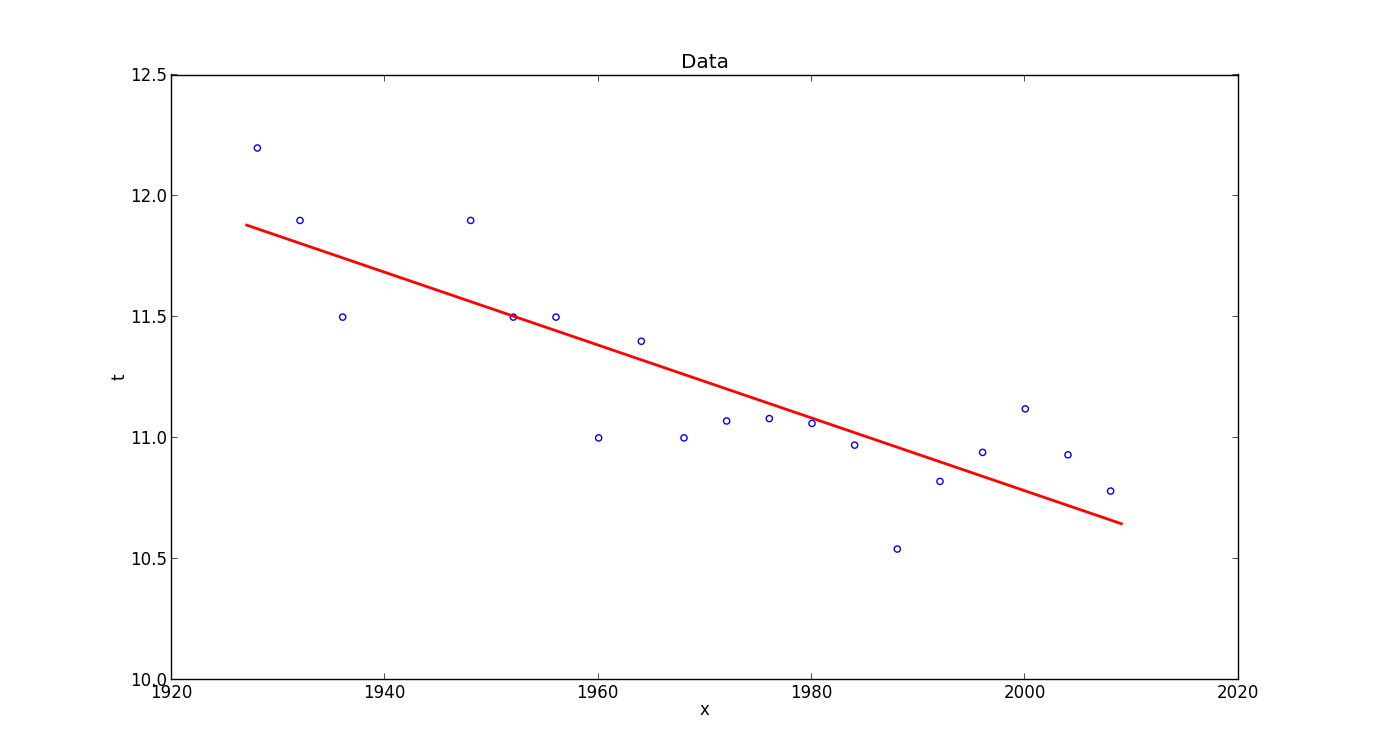
\includegraphics[width=12cm]{figs/figure_1.png}
\caption{Solution: 1st-order polynomial model}
\end{center}
\end{figure}


%%%     Problem 3
\item[3.] [1 point]
Adapted from {\bf Exercise 1.7} of FCMA p.35:

Using the model obtained in the previous exercise, predict the women's winning time at the 2012 and 2016 Olympic games; report the values here.  What is the squared error of your model's prediction for Shelly-Ann Fraser-Price's gold medal time of 10.75 seconds in the 2012 Olympics women's 100m race?

{\bf Solution:} Substituting $x = 2012$ in our model equation, we will have:

$t_{2012} =  40.924 -0.015*2012 = 10.74$

$t_{2016} =  40.924 -0.015*2016 = 10.68$

$\epsilon_{2012} = (10.75 - 10.74)^{2} = 0.01^{2} = 10^{-4}$


%%%     Problem 4
\item[4.] [1 point]
Adapted from {\bf Exercise 1.9} of FCMA p.36:

Use your python script from problem 1 to load the data stored in the file {\tt synthdata2014.csv} (in the data folder).  Fit a 3rd order polynomial function -- $f(x; \mathbf{w}) = w_0 + w_1 x + w_2 x^2 + w_3 x^3$ -- to this data (if you extended the {fitpoly\_incomplete.py} script, then {\tt model\_order}$ = 3$).  
Present and describe the parameters you obtain fitting to this data.  Also, plot the data and your linear-fit model and include the plot in your answer.

{\bf Solution:} According to the output of our model, we have:

\begin{verbatim}
[emanuel@localhost scripts]$ python exer4.py 
Identified model parameters:
[[  9.02190177]
 [  4.54356124]
 [ 49.43723008]
 [  5.00595904]]
\end{verbatim}

So, the parameters are:

$w_{0} = 9.02190177, w_{1} = 4.54356124, w_{2} = 49.43723008,$ and $w_{3} = 5.00595904 $

\begin{figure}[htb]
\begin{center}
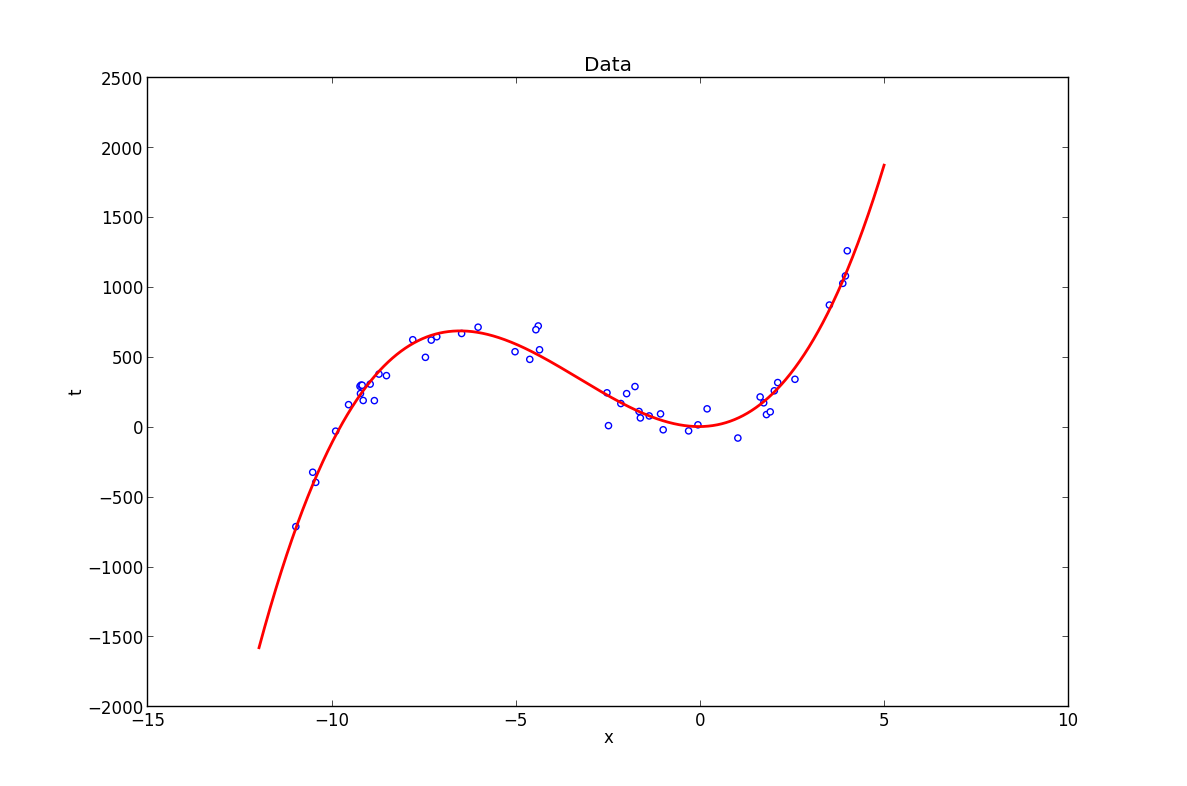
\includegraphics[width=10cm]{figs/figure_4.png}
\caption{Solution: 3rd-order polynomial model fitting data}
\end{center}
\end{figure}




%%%     Problem 5
\item[5.] [3 points]
Write a script that implements K-fold cross-validation to choose the polynomial order (between orders 0 and 7) with the best predictive error for the {\tt synthdata2014.csv}.  The provided script {\tt cv\_demo\_incomplete.py} implements the synthetic data experiment described in Ch 1 (pp.31-32) of the book; you are welcome to use and adapt any part of this code you like; keep in mind that this script won't successfully execute until you add the general (matrix form) normal equation calculation on line 81.
Note also that in the synthetic data experiment in {\tt cv\_demo\_incomplete.py}, 1000 test data points are generated in addition to the 100 data points used for 10-fold cross-validation; for problem 5, you won't have this independent test set, only the data from {\tt synthdata.csv} on which to perform K-fold cross-validation.

Run your script with 10-fold cross-validation and Leave-One-Out-CV (LOOCV).
Which model order do the two cross-validation methods predict as the best order for predictive accuracy?
Do the two different cross-validation runs agree?

Report the best-fit model parameters for the best model order according to 10-fold CV, and plot this model with the data.
Include a plot of the CV-loss and training loss for the 8 different (0..7) polynomial model orders for both the 10-fold cross-validation and for LOOCV.

You will submit your script as a stand-alone file called {\tt cv.py}

{\bf Solution:}  According to the model developed, both cross-validation methods runs agree and the best model order for both was 3. 

The best fit model parameters (model order 3) are:

$w_{0} = 9.13981397, w_{1} =  4.46592473, w_{2} =  49.41560256 ,$ and $w_{3} =  5.00477336 $

and the data will be fit as following:

          
\begin{figure}[htb]
\begin{center}
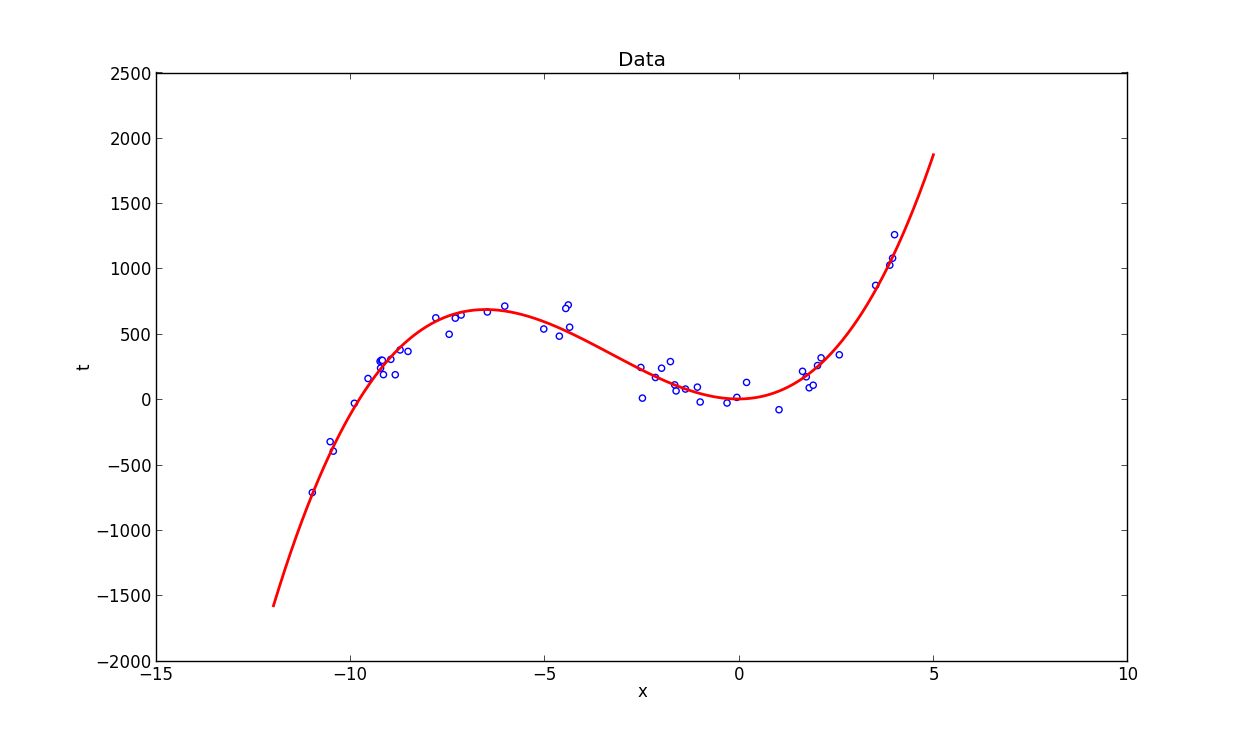
\includegraphics[width=10cm]{figs/figure_5.png}
\caption{Solution: Best fit model parameters (model order = 3)}
\end{center}
\end{figure}


     
\begin{figure}[htb]
\begin{center}
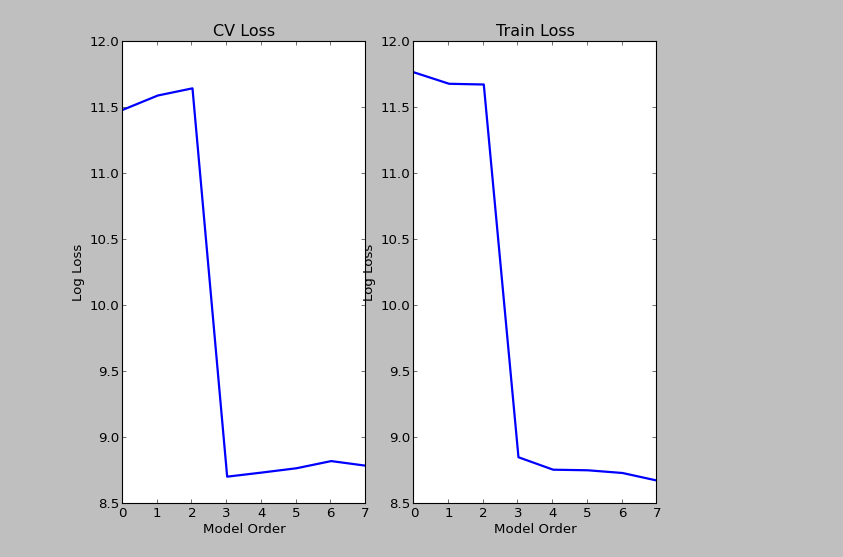
\includegraphics[width=10cm]{figs/figure_5k10.png}
\caption{Solution: CV-loss and training loss for the 8 different (0..7) polynomial model orders - CV, K = 10}
\end{center}
\end{figure}
     
\begin{figure}[htb]
\begin{center}
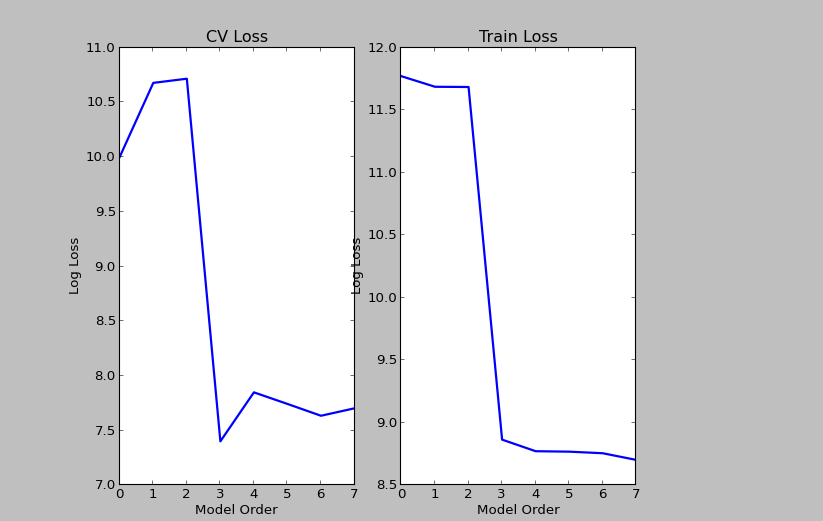
\includegraphics[width=10cm]{figs/figure_5k50.png}
\caption{Solution: CV-loss and training loss for the 8 different (0..7) polynomial model orders - LOOCV, K = 50}
\end{center}
\end{figure}


\newpage

%%%     Problem 6
\item[6.] [2 points -- {\bf Required only for Graduates}] 
{\bf Exercise 1.10} from FCMA p.36

Derive the optimal least squares parameter value, $\mathbf{\hat{w}}$, for the total training loss:
\begin{eqnarray*}
\mathcal{L} = \sum_{n=1}^N \left( t_n - \mathbf{w}^\top \mathbf{x}_n \right)^2
\end{eqnarray*}

How does the expression compare with that derived from the average (mean) loss?  (Hint: Express this loss in the {\bf full} matrix form and derive the normal equation.)

{\bf Solution:} Let us express $\mathcal{L} $ in the full matrix form: Suppose we have one target (one column) vector $\mathbf{t}$, one design matrix (2 column) $\mathbf{X}$, and one parameter vector $\mathbf{w}$. So, we have:

\begin{eqnarray*}
\mathbf{t - Xw}  = 
    \begin{bmatrix}
    t_{1} - w_{0}  - w_{1}x_{1}\\[0.3em]
    t_{2} - w_{0}  - w_{1}x_{2}\\[0.3em]
    \vdots \\[0.3em]
    t_{n} - w_{0}  - w_{1}x_{n}\\[0.3em]
    
    \end{bmatrix}
\end{eqnarray*}

Now, we will use a single multiplication and transpose to neatly perform the squaring and summation and obtain our original loss funcion $\mathcal{L}$:

$\mathbf{(t - Xw)}^\top \mathbf{(t - Xw)} = (w_{0} + w_{1}x_{1} -t_{1})^{2} + (w_{0} + w_{1}x_{2} -t_{2})^{2} + \hdots + 
(w_{0} + w_{1}x_{n} -t_{n})^{2} =$\\
$= \sum_{n=1}^N ( w_{0} + w_{1}x_{n} -t_{n})^2 = \sum_{n=1}^N (t_{n} - f(x_{n}; w_{0}, w_{1}))^2$  

Thus, our loss function in full matrix notation will be:

$\mathcal{L} = (\mathbf{t - Xw})^\top (\mathbf{t - Xw})$

Applying the distributing and transpose property in $\mathcal{L}$:

$\mathcal{L} = (\mathbf{(t^\top  - w^\top X^\top) (t - Xw)  }) = $ \\
$ = \mathbf{(t^{\top}t -t^{\top}Xw - w^{\top}X^{\top}t + wX^{t}Xw})$ 

The two terms $\mathbf{-t^{\top}Xw}$ and $\mathbf{ w^{\top}X^{\top}t}$ are the transpose of one another and also scalars. Therefore, 
they can be combined, so:

$\mathcal{L} = \mathbf{(t^{\top}t -2t^{\top}Xw  + wX^{t}Xw})$ 

Differentiating $\mathcal{L}$ and setting to zero:

 $\frac{\partial \mathcal{L}}{\partial \mathbf{w}} = \mathbf{-2X^{\top}t + 2X^{\top}Xw} = 0 =>$ \\
 $=>  \mathbf{X^{\top}Xw = X^{\top}t} => \mathbf{(X^{\top}X)^{-1} X^{\top}Xw = (X^{\top}X)^{-1} X^{\top}t}$
 
However, we know that $\mathbf{(X^{\top}X)^{-1} X^{\top}X} = \mathbb{I} $. Therefore:

$\mathbf{\mathbb{I}w = (X^{\top}X)^{-1} X^{\top}t} $ \\ [0.5 cm]

Therefore, $\mathbf{\hat{w}} = \mathbf{(X^{\top}X)^{-1} X^{\top}t} $





%%%     Problem 7
\item[7.] [2 points -- {\bf Required only for Graduates}]
{\bf Exercise 1.11} from FCMA p.36

The following expression is known as the {\em weighted} average loss:
\begin{eqnarray*}
\mathcal{L} = {1 \over N} \sum_{n=1}^N \alpha_n \left( t_n - \mathbf{w}^\top \mathbf{x}_n \right)^2
\end{eqnarray*}

where the influence of each data point is controlled by its associated parameter.  Assuming that each $\alpha_n$ is fixed, derive the optimal least squares parameter value $\mathbf{\hat{w}}$.  (Hint: When expressing in the full matrix form, the $alpha$'s become a matrix...)

{\bf Solution:} Before writing $\mathcal{L}$ in the full matrix form, we will define the matrix $\alpha$ as $A$ as follows:

$A = 
\begin{bmatrix}
\alpha_{1} &  0  & \ldots & 0\\
0  &  \alpha_{2} & \ldots & 0\\
\vdots & \vdots & \ddots & \vdots\\
0  &   0       &\ldots &\alpha_{n}
\end{bmatrix}
$

Using the same process we took in the previous exercise, we can write $\mathcal{L}$ as follows:

$\mathcal{L} = \frac{1}{N}((\mathbf{t - Xw})^\top A(\mathbf{t - Xw}))$

Doing this way, we can guarantee that we will have one $\alpha_{n}$ for each data point. Now, we will do the same process 
we used in the previous exercise. We will apply the distributing property in $\mathcal{L}$ :

$\mathcal{L} = \frac{1}{N}(\mathbf{(t - Xw)^{\top} (At - AXw})) = $ \\
$= \frac{1}{N}(\mathbf{(t^{\top} - (Xw)^{\top}) (At - AXw})) =$ \\
$= \frac{1}{N}(\mathbf{t^{\top}At - t^{\top}AXw - (Xw)^{\top}At + (Xw)^{\top}AXw}) $ \\

The two terms $\mathbf{t^{\top}AXw}$ and $\mathbf{(Xw)^{\top}At}$ are the transpose of one another and also scalars. Therefore, 
they can be combined, so:

$\mathcal{L}= \frac{1}{N}(\mathbf{t^{\top}At - 2(Xw)^{\top}At + (Xw)^{\top}AXw}) = $ \\
$ \frac{1}{N}(\mathbf{t^{\top}At - 2w^{\top}X^{\top}At + (Xw)^{\top}AXw}) $ \\

Differentiating $\mathcal{L}$ and setting to zero:

$\frac{\partial \mathcal{L}}{\partial \mathbf{w}} = \mathbf{-2X^{\top}At + 2X^{\top}AXw} = 0 =>$ \\
$\mathbf{X^{\top}AXw = X^{\top}At } => \mathbf{(X^{\top}AX)^{-1} X^{\top}AXw = (X^{\top}AX)^{-1} X^{\top}At } =>$  \\
$\mathbf{\mathbb{I} w = (X^{\top}AX)^{-1} X^{\top}At }$ \\[0.5 cm]

Therefore, $\mathbf{ \hat{w} = (X^{\top}AX)^{-1} X^{\top}At }$








%%%     Problem 8
\item[8.] [4 points]
Variant of {\bf Exercise 1.12} from FCMA p.36

Write a new Python script that uses $K$-fold cross-validation to find the value of $\lambda$ that gives the (approximate) best predictive performance on the synthetic data ({\tt synthdata.csv}) using {\bf regularized} least squares with a {\bf 7th order polynomial} model.  Report here the lambda you identified, the best fit linear model using that lambda (as a linear equation) and include a plot of the MSE loss as a function of $\lambda$ that shows the loss curve with a minimum, and a plot of the best-fit model with the data.

You will submit the script as a stand-alone file called {\tt regularize.py}.

{\bf Solution:} The best lambda identified was $0.1$. According to the output of our model:

\begin{verbatim}
emanuel@localhost submit]$ python regularize.py 
Best parameters considering best lambda =  0.1 are: 
[  7.80554395e+00   4.00116996e+00   4.57982000e+01   1.13186782e+00
  -1.12223146e-01   2.33469379e-01   3.61837459e-02   1.51821005e-03]

\end{verbatim} 

The parameters are:

$\mathbf{ \hat{w} }=\begin{bmatrix}
w_{0}\\
w_{1}\\
\vdots \\
w_{7}
\end{bmatrix} = $
$\begin{bmatrix}
7.80554395e+00\\
4.00116996e+00\\
4.57982000e+01\\
1.13186782e+00\\
-1.12223146e-01   \\
2.33469379e-01\\
3.61837459e-02\\
1.51821005e-03\\
\end{bmatrix}$

        
\begin{figure}[htb]
\begin{center}
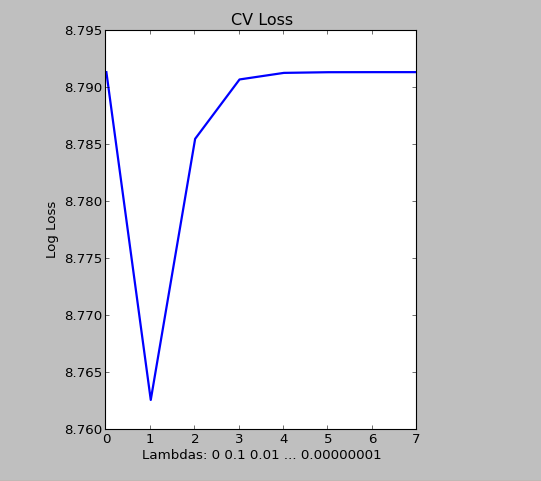
\includegraphics[width=10cm]{figs/figure_8b.png}
\caption{MSE loss as a function of $\lambda$. Each integer in X-axis is the index of lambda array. The lambada array is [0, 0.1, 0.01, 0.001, 0.0001, 0.00001, 0.000001, 0.0000001]}
\end{center}
\end{figure}


\begin{figure}[htb]
\begin{center}
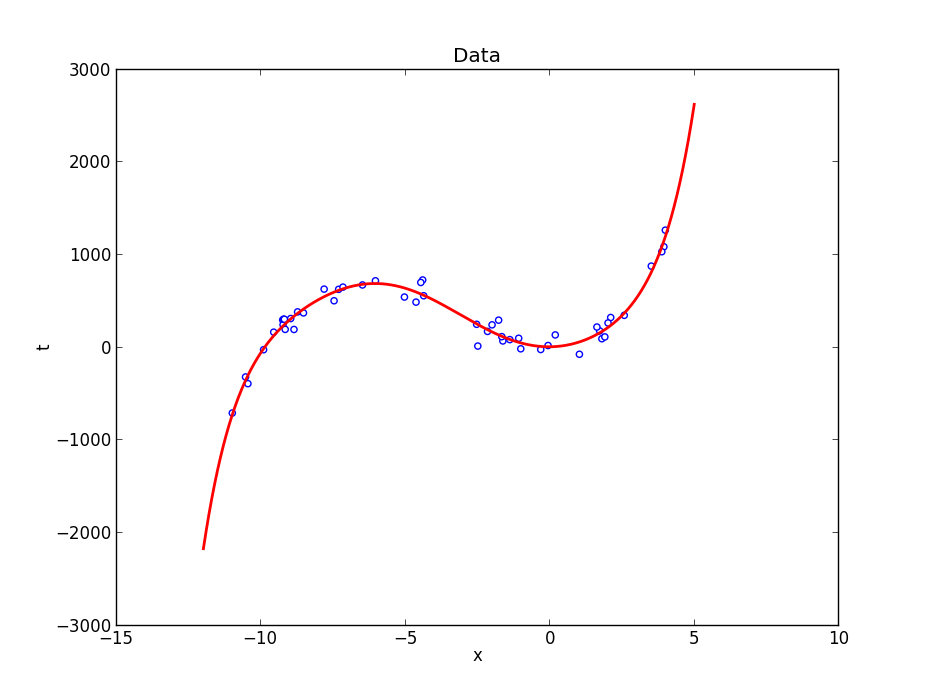
\includegraphics[width=10cm]{figs/figure_8.png}
\caption{Best fit model: lambda = 0.1, model order = 7, CV k=10}
\end{center}
\end{figure}
\end{itemize}

\end{document}